\section{Organizacja} 
\begin{figure}[H]
\centering
 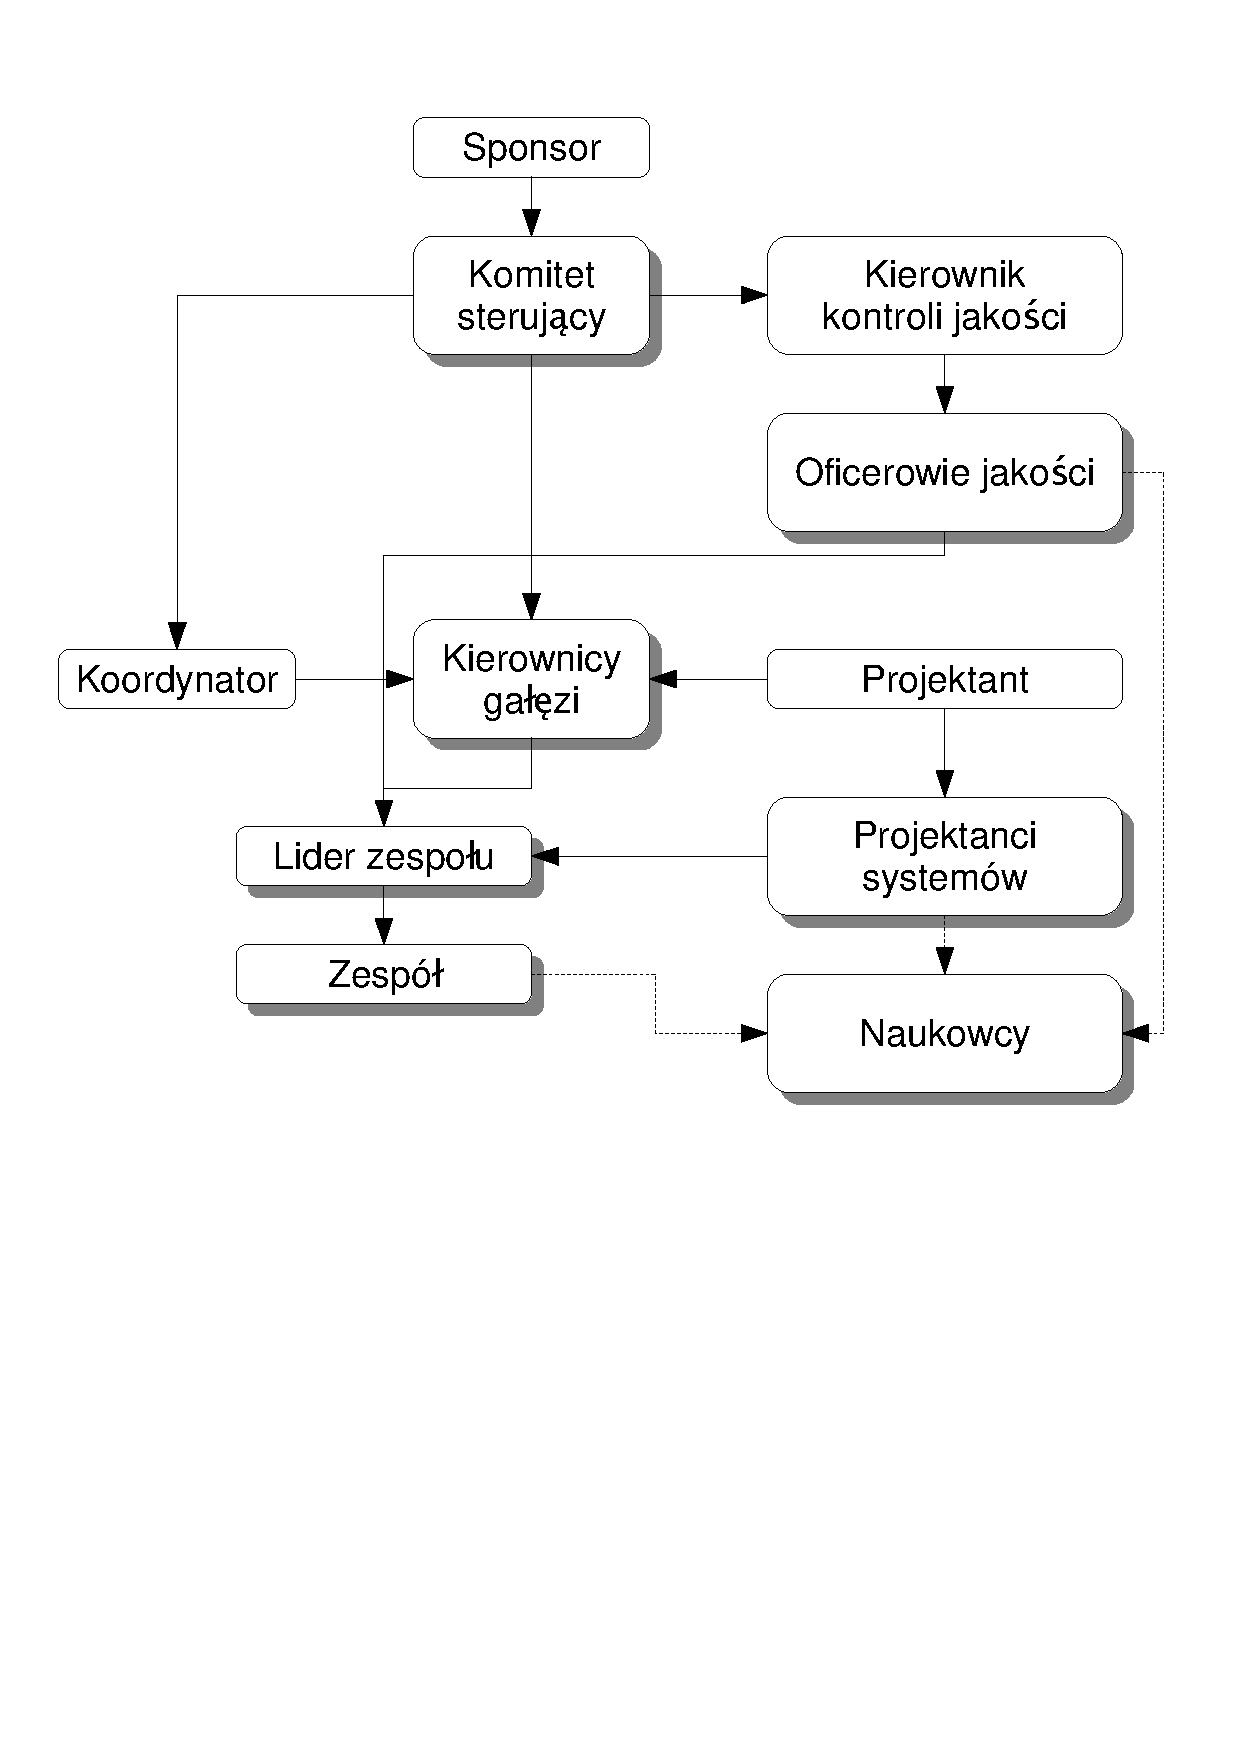
\includegraphics[width=\textwidth]{img/struktura.pdf}
\caption{Zarys zależności stanowisk projektu.}
\end{figure}
\subsection{Sponsor}
Sponsorem będzie prezydent Islandii.
Będzie on zarządzał finansowaniem projektu, oraz wyznaczał ogólne wytyczne.

Będzie bezpośrednio brał udział w rozmowach z największymi sponsorami, wyznaczał kształt zarządu, oraz sprawował ogólną władzę nad wszystkim.
Każda jego decyzja będzie jawna publicznie.

\subsection{Komitet sterujący}
Powołani przez prezydenta ministrowie będą decydować o ogólnym kierunku projektu i przeprowadzać kontrole pomiędzy etapami.

W skład komitetu wejdą również najwięksi sponsorzy, których wpływ na podejmowanie decyzji będzie zależny od wniesionego wkładu.

\subsection{Kierownicy gałęzi}
Kierownicy będą powoływani przez komitet sterujący, każdy specjalizował się będzie w innej dziedzinie i zarządzał znanymi dla siebie zespołami.

Każdy z kierowników będzie miał pod sobą określone dla swojej specjalizacji zespoły i będzie odpowiadał za to, aby określona część infrastruktury została zbudowana zgodnie z planem, budżetem i jakością.
Do pomocy w pracy będzie mógł zaprosić projektantów i naukowców.

\subsection{Koordynator}
Ponieważ planowany jest udział wielu kierowników, z których każdy zajmie się swoją dziedziną, istnieje potrzeba stworzenia stanowiska pośredniczącego między nimi.
Koordynator będzie się zajmował się dialogiem pomiędzy kierownikami, aby odpowiednio zarządzali częściami dla siebie wspólnymi.
Będzie miał także bezpośredni kontakt z komitetem sterującym oraz będzie mógł zwrócić się o pomoc do projektanta.

\subsection{Główny projektant}
Będzie nadzorował cały projekt pod kątem ogólnym. 
Nie będzie w stanie samodzielnie ogarnąć wszystkich dziedzin, dlatego będzie miał pod sobą zespół projektantów systemowych.

Projektant będzie współpracował z koordynatorem i kierownikami gałęzi.

\subsection{Projektanci systemowi}
Projektant główny nie będzie w stanie zaprojektować sam całego przedsięwzięcia.
Do tego potrzebna jest właśnie grupa projektantów z których każdy jest wyspecjalizowany w innej dziedzinie.
Oprócz tego, do dyspozycji są też dostępni projektanci odpowiedzialni za logistykę i sposób budowy tego, co zaprojektowali inni.

Do projektantów zgłaszają się liderzy zespołów w razie niejasności w planie.
Gdyby projektanci mieli jakieś problemy, to mają do pomocy grupę naukowców, którzy pomogą im w podejmowaniu decyzji.

\subsection{Naukowcy}
Grupa naukowców zostanie powołana przez komitet sterujący.
Na grupę złożą się doradcy ministrów, pracownicy laboratoriów sponsorów, oraz grupy zgłoszone przez różne uczelnie świata.

Zadaniem naukowców będzie udzielanie specjalistycznej pomocy (w szczególności projektantom), prowadzenie badań i wykonywanie najbardziej skomplikowanych prac. 
Będą więc mieli pośredni wpływ na to, jaka powinna być jakość projektowanych systemów i jak je zaprojektować.
Projektanci, oficerowie i niektórzy liderzy zespołów będą mogli korzystać z ich pomocy zarówno teoretycznej, jak i praktycznej.

\subsection{Rekruterzy}
Spośród grupy naukowców wyznaczane będą kilkuosobowe zespoły, odpowiedzialne za rekrutację zespołów wykonawczych. Będą oni decydowali o liczebności przyjmowanych zespołów i sprawdzali kwalifikacje kandydatów.

\subsection{Kierownik kontroli jakości}
Powołany przez komitet sterujący będzie ich wysłannikiem kontrolującym przebieg procesu budowy oraz utrzymania systemu.
Z pomocą swoich oficerów będzie sprawdzał, czy odpowiednie części projektu są tworzone zgodnie z założeniami i czy kierownicy należycie kontrolują poczynania swoich podwładnych.

Swój raport będzie zgłaszał do komitetu sterującego.

\subsection{Oficerowie jakości}
Ta grupa zarządzana będzie przez kierownika kontroli jakości.
Każdy z oficerów będzie się specjalizował w innej dziedzinie.
Razem z odpowiednim dla siebie kierownikiem gałęzi i projektantem systemowym będą uczestniczyć w okresowych kontrolach zespołów.
Swoje uwagi będą zgłaszać kierownikowi kontroli jakości.

\subsection{Zespoły wykonawcze}
Każdy zespół będzie się składał się z wyselekcjonowanych przez dbającą o odpowiednie kwalifikacje grupę rekruterów.
Zakłada się możliwość zbiorczego przyjęcia całego zespołu, gdy na przykład w tym samym składzie pracował wcześniej w innej firmie.
Prawdopodobnie wiele zespołów zostanie zgłoszonych przez sponsorów.

Każdy zespół zajmie się małym fragmentem projektu. Na przykład jeden zespół może zająć się budową odcinka toru dla wewnętrznego transportu, inny zwrotnicami.
Jeden zespół będzie ustawiał bramki do sprawdzania pojazdów na nadajniku, a inny projektował moduł sterowników do obsługi jednego z kryształów.

Każdy zespół będzie miał swojego lidera, który uczestniczyć będzie w przekazywaniu informacji wyżej.

\subsection{Lider zespołu}
Obowiązkiem lidera zespołu będzie dobra orientacja w przebiegu pracy zespołu, znajomość postępów prac i występujących problemów. 
Będzie on raportował do kierownika odpowiedniej gałęzi projektu i przyjmował okresowe kontrole.

W razie problemów w wykonywaniu planu będzie się zgłaszał o pomoc do swojego projektanta systemowego, a w przypadku poważniejszych problemów także do grupy naukowców.

Lider będzie mógł zgłosić zapotrzebowanie na udział w pracy swojego zespołu któregoś z naukowców w celu wykonania zaawansowanych prac, albo bezpośrednio zgłosić się o pomoc w niewielkim zakresie przy wykonywaniu prac.

\subsection{Zasoby materialne}
W początkowych fazach projektu powstanie niewielkie miasteczko pracownicze wokół całej planowanej struktury. Docelowo powstaną tam również hotele, centra rozrywki, biurowce itp.

Infrastruktura telekomunikacyjna powinna być zbudowana jako jedna z pierwszych, bo to na niej bazują pracownicy. Niezbędny będzie szybki internet, stąd budowa odpowiedniej sieci powinna być priorytetem od początku powstawania miasteczka.

Pracownicy, którzy będą budować te struktury, początkowo zamieszkają w barakach z kontenerów. Potem w miarę rozwoju będą mogli się przenosić do kolejnych budynków o wyższym standardzie.

Wtedy też dołączą bardziej wykwalifikowani pracownicy, którzy mieszkając w hotelach i pracując w biurach będą zajmować się innymi częściami projektu.

Do czasu ukończenia budynków mieszkalnych w bezporedniej bliskości Centrali, zarząd stacjonować będzie w Reykjaviku, wysyłając często pojedyncze osoby do kontroli prac budowlanych. Potem wszyscy powinni przenieść się na miejsce, aby dokładnie kontrolować postęp.

\subsection{Centrala}
Główne biuro projektu z którego wysyłane będą osoby i komunikaty.
To tam będą się zgłaszać liderzy zespołów w razie problemów i tam znajdą się sale konferencyjne.

W najbliższej okolicy centrali, w celu umożliwienia szybkiej komunikacji, powinny mieszkać osoby z zarządu.

Będzie to miejsce, gdzie znajdą się biura projektowe i gdzie będą stacjonować naukowcy.

\subsection{Węzeł komputerowy}
Zespoli ze sobą cały projekt, służąc za źródło informacji nie tylko w sferze projektowej, lecz także do komunikacji między pracownikami i zarządem.

To właśnie tam odpowiednie osoby zgłaszać będą swoje raporty, a ich kierownicy będą mogli je przeczytać.
Tam wyznaczane będą terminy spotkań i kontroli i rozsyłane o nich informacje.